\chapter{Implementación del sistema basado en IoT}\label{cap: }

\addcontentsline{toc}{section}{Introducción}
        \textbf{\Large Introducción}\newline
        ...

\section{Descripción técnica capa de percepción}

Como se analizaba en el epígrafe \ref{subsec:capa_percepcion} la capa de percepción va caracterizada por la presencia del microcontrolador y los sensores que, en conjunto forman los nodos, siendo estos los
encargados de la captura de los datos del medio.\\

Los nodos están diseñados sobre una placa de circuito impreso PCB (figura \ref{imag:pcb_nodo}) en la que se hizo el montaje de los componentes.
El diseño está pensado para con el menor consumo posible recopilar la mayor cantidad de información.

\begin{figure}[H]
    \centering
    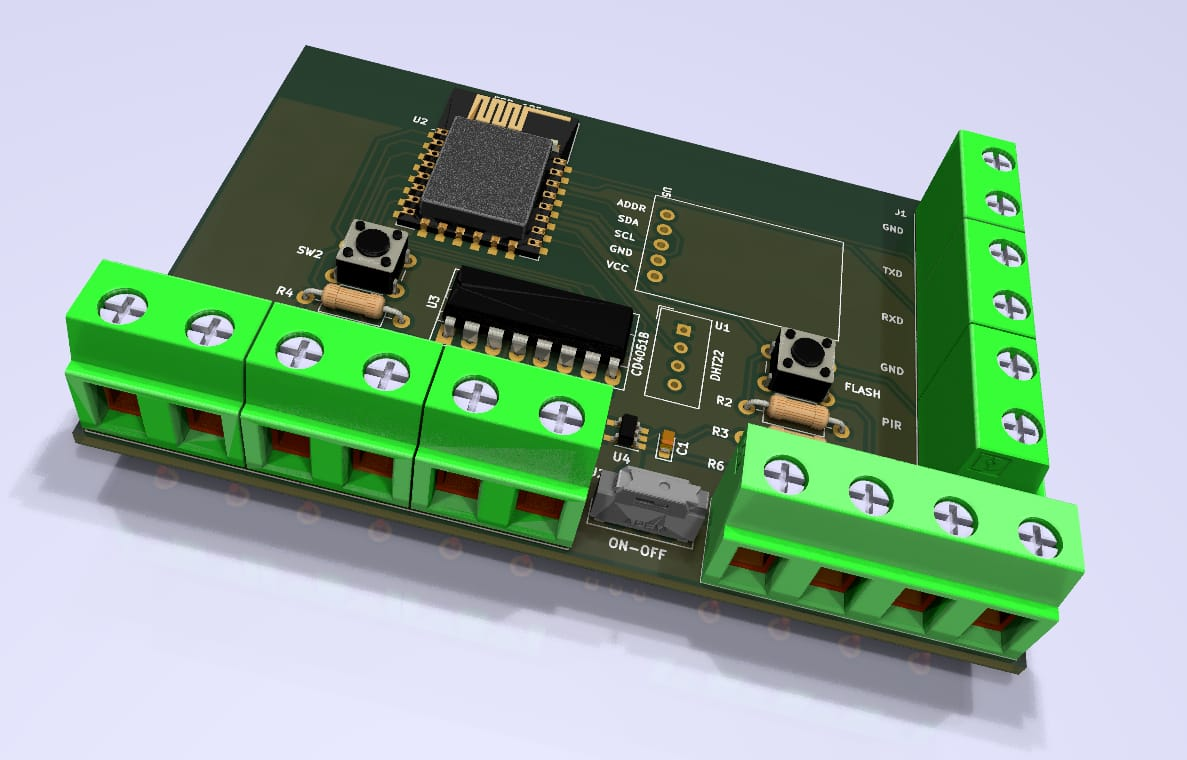
\includegraphics[width=6cm, height=4cm]{imagenes/vista 3D.jpg}
    \caption{PCB Nodo}
    \subcaption*{Fuente: Elavoración propia}
    \label{imag:pcb_nodo}
\end{figure}

\begin{figure}[H]
    \centering
    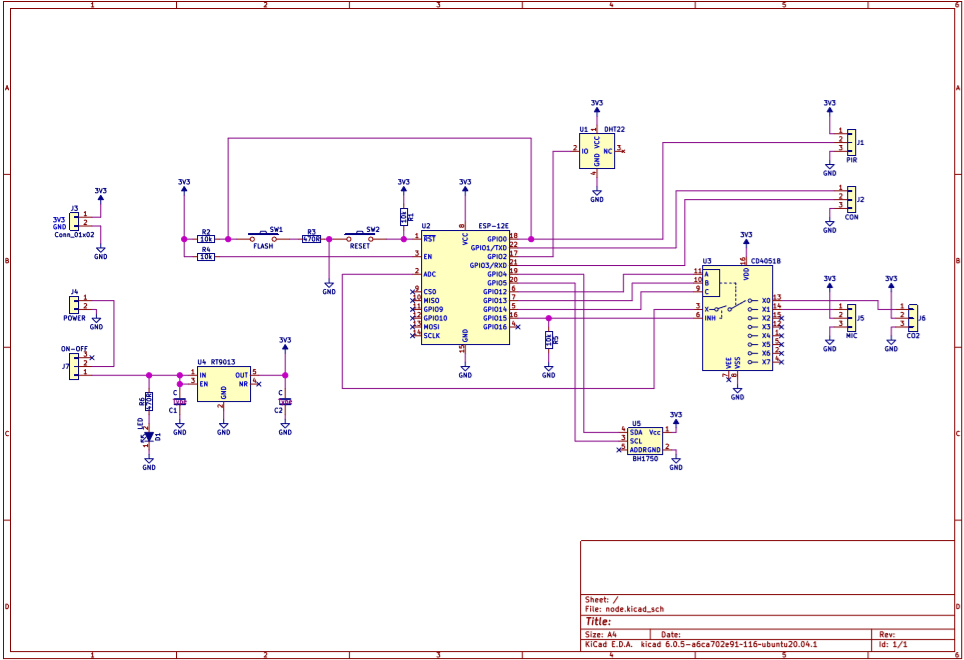
\includegraphics[width=12cm, height=8cm]{imagenes/esquematico nodo.jpg}
    \caption{Esquematico del circuito}
    \subcaption*{Fuente: Elavoración propia}
    \label{imag:esquematico_nodo}
\end{figure}

A continuación se describen por partes los elementos que componen dichos nodos.


\subsection{Microcontrolador} \label{sec: microcontrolador}

    Un microcontrolador (abreviado: MCU) es un circuito integrado programable, capaz de ejecutar las órdenes grabadas en su memoria. Está compuesto de varios bloques funcionales, los cuales cumplen una tarea específica. Un microcontrolador incluye en su interior las tres principales unidades funcionales de una computadora: unidad central de procesamiento, memoria y periféricos de entrada/salida.\\

The ESP-12F WiFi module was developed by Ai-Thinker Technology. The core processor
ESP8266 integrates the industry-leading Tensilica L106 ultra-low-power 32-bit micro MCU in
a small package with 16-bit Lite mode, clocked at Supports 80 MHz and 160 MHz, supports
RTOS, and integrates Wi-Fi MAC/BB/RF/PA/LNA.

The ESP-12F WiFi module supports the standard IEEE802.11 b/g/n protocol, a complete
TCP/IP protocol stack. Users can use this module to add networking capabilities to existing
devices or to build separate network controllers.

The ESP8266 is a high-performance wireless SOC that offers maximum utility at the lowest
cost and unlimited possibilities for embedding WiFi functionality into other systems.

The ESP8266 is a complete and self-contained WiFi network solution that can operate
independently or as a slave running on other host MCUs. The ESP8266 is capable of booting
directly from an external flash memory when it is powered by an application and is the only
application processor in the device. The built-in cache helps improve system performance and
reduce memory requirements.

In another case, the ESP8266 is responsible for wireless Internet access. When it comes to
the task of the WiFi adapter, it can be added to any micro controller-based design. The connection
is simple and easy, just by SPI / SDIO interface or I2C / UART port. Just fine.

The ESP8266's powerful on-chip processing and storage capabilities allow it to integrate
sensors and other application-specific devices through the GPIO port, minimizing system
resources during minimal up-front development and operation. \cite{esp12}.\\

    El microcontrolador ESP-12F de Ai-Thinker (Figura \ref{imag:esp-12F}), basado en ESP8266.

    \begin{figure}[H]
        \centering
        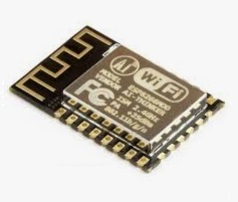
\includegraphics[width=4cm, height=4cm]{imagenes/esp-12F.jpeg}
        \caption{ESP-12F}
        \label{imag:esp-12F}
    \end{figure}

    \textbf{Características}

    \begin{itemize}
        \item The smallest 802.11b/g/n Wi-Fi SOC module
        \item Low power 32-bit CPU, can also serve as the application processor
        \item Up to 160MHz clock speed
        \item Built-in 10 bit high precision ADC
        \item Supports UART/GPIO/IIC/PWM/ADC
        \item SMD-22 package for easy welding
        \item Integrated Wi-Fi MAC/BB/RF/PA/LNA
        \item Support multiple sleep patterns. Deep sleep current as low as 20uA
        \item UART baud rate up to 4Mbps
        \item Embedded LWIP protocol stack
        \item Supports STA/AP/STA + AP operation mode
        \item Support Smart Config/AirKiss technology
        \item Supports remote firmware upgrade (FOTA)
        \item General AT commands can be used quickly
    \end{itemize}

    \begin{figure}[H]
        \centering
        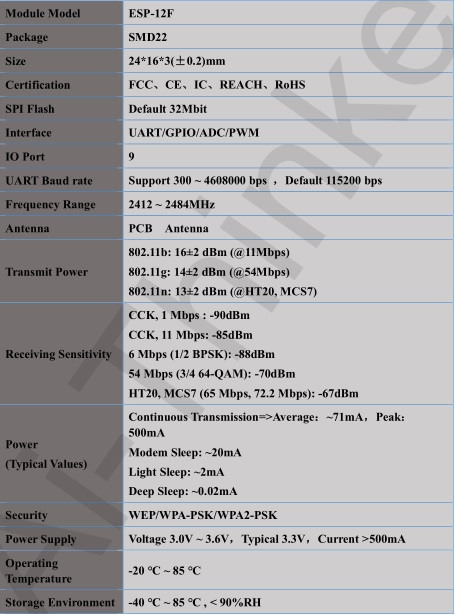
\includegraphics[width=10cm, height=13cm]{imagenes/esp-12F especificaciones.jpg}
        \caption{Especificaciones ESP-12F}
        \subcaption*{Fuente: Datasheet fabricante}
        \label{imag:esp-12F_especificaciones}
    \end{figure}

    
    \begin{figure}[H]
        \centering
        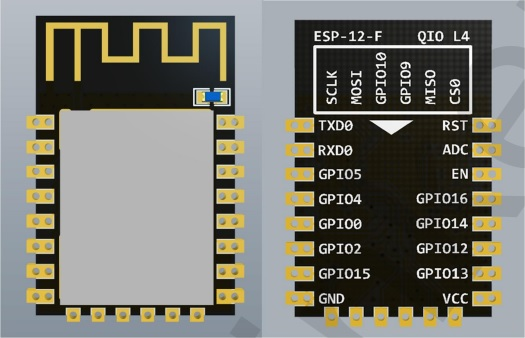
\includegraphics[width=6cm, height=4cm]{imagenes/esp-12F pinout.jpg}
        \caption{ESP-12F Pinout}
        \subcaption*{Fuente: Datasheet fabricante}
        \label{imag:esp-12F_pinout}
    \end{figure}

    \begin{figure}[H]
        \centering
        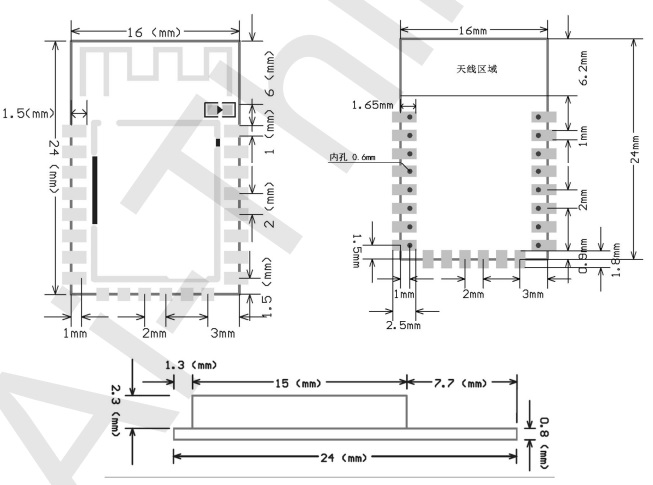
\includegraphics[width=10cm, height=7cm]{imagenes/esp-12F dimensiones.jpg}
        \caption{ESP-12F Dimensiones}
        \subcaption*{Fuente: Datasheet fabricante}
        \label{imag:esp-12F_dimensiones}
    \end{figure}

    \vspace{4cm}

    %Dentro de la familia de los ESP se encuentra el NodeMCU. Este microcontrolador (Imagen \ref{imag:nodemcu}) será el encargado de recibir los datos de los sensores y organizarlos en función de su continua transmisión hacia el concentrador.\\

    %\begin{figure}[h]
    %    \centering
    %    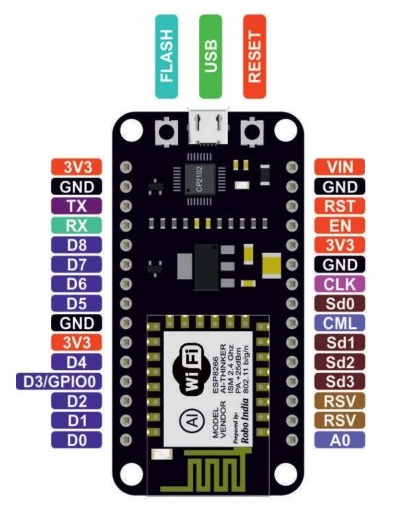
\includegraphics[width=5.5cm, height=6cm]{imagenes/nodemcu0.jpg}
    %    \caption{NodeMcu Vendor}
    %    \label{imag:nodemcu}
    %\end{figure}
    
    
    %NodeMCU es una pequeña placa Wifi compatible con Arduino, lista para usar en cualquier proyecto IoT. Está montada alrededor del microcontrolador ESP8266 y expone todos sus pines en los laterales. Además, ofrece más ventajas como la incorporación de un regulador de tensión integrado, así como un puerto USB de programación. Se puede programar con LUA o mediante el IDE de Arduino.\\

    %Dispone de una extensa comunidad y documentación que permitirá conectar el proyecto mediante conexión Wifi.

    %\textbf{Características}
    %\begin{itemize}
    %    \item Procesador: ESP8266 a 80MHz (3.3V) (ESP-12E).
    %    \item 4MB de memoria FLASH (32 MBit).
    %    \item WiFi 802.11 b/g/n.
    %    \item Regulador 3.3V integrado (500mA).
    %    \item Conversor USB-Serial CH340G.
    %    \item Función Auto-reset.
    %    \item 9 pines GPIO con I2C y SPI.
    %    \item 1 entrada analógica (1.0V max).
    %    \item 4 agujeros de montaje (3mm).
    %    \item Entrada alimentación externa VIN (20V max).
    %\end{itemize}

\subsection{Sensores} \label{sec: sensores}

    La secuencia de sensores pertenecientes al sistema es selecta, puesto que se tomaron los sensores teniendo en cuenta varios factores:

    \begin{itemize}
        \item Variable a medir
        \item Rango de operación
        \item Precisión
        \item Voltaje de alimentación
        \item Corriente de alimentación
        \item Precio
    \end{itemize}

    \vspace{3cm}

En la siguiente tabla se relacionan los mismos.

\begin{table}[H]
    \centering
    \caption{Relación sensores}
    \subcaption*{Fuente: Elaboración propia}
    \begin{tabular}{|c|c|c|cccc|}
    \hline
    \rowcolor[HTML]{9698ED} 
    \cellcolor[HTML]{9698ED}                      & \cellcolor[HTML]{9698ED}                                        & \cellcolor[HTML]{9698ED}                         & \multicolumn{4}{c|}{\cellcolor[HTML]{9698ED}Características}                                                                                                                                                                                                                          \\ \cline{4-7} 
    \rowcolor[HTML]{9698ED} 
    \multirow{-2}{*}{\cellcolor[HTML]{9698ED}No.} & \multirow{-2}{*}{\cellcolor[HTML]{9698ED}Variable}              & \multirow{-2}{*}{\cellcolor[HTML]{9698ED}Nombre} & \multicolumn{1}{c|}{\cellcolor[HTML]{9698ED}Rango}                                           & \multicolumn{1}{c|}{\cellcolor[HTML]{9698ED}Precisión} & \multicolumn{1}{c|}{\cellcolor[HTML]{9698ED}\begin{tabular}[c]{@{}c@{}}Voltaje\\ alimentación\end{tabular}} & Corriente       \\ \hline
    1                                             & \begin{tabular}[c]{@{}c@{}}Temperatura y\\ Humedad\end{tabular} & DHT22                                            & \multicolumn{1}{c|}{\begin{tabular}[c]{@{}c@{}}De - 40 a 80°C y\\ De 0 a 100RH\end{tabular}} & \multicolumn{1}{c|}{5\%}                               & \multicolumn{1}{c|}{De 3v a 6v}                                                                             & 2.5mA           \\ \hline
    2                                             & CO2                                                             & MH-Z19C                                          & \multicolumn{1}{c|}{\begin{tabular}[c]{@{}c@{}}De 400ppm a\\ 5000ppm\end{tabular}}           & \multicolumn{1}{c|}{5\%}                               & \multicolumn{1}{c|}{5v}                                                                                     & \textless{}40mA \\ \hline
    3                                             & Vibración                                                       & M0168                                            & \multicolumn{1}{c|}{\begin{tabular}[c]{@{}c@{}}Salida analógica\\ (0-1024)\end{tabular}}     & \multicolumn{1}{c|}{2\%}                               & \multicolumn{1}{c|}{De 3.3v a 5v}                                                                           & \textless{}10mA \\ \hline
    4                                             & Polución                                                        & SDS011                                           & \multicolumn{1}{c|}{\begin{tabular}[c]{@{}c@{}}De 0.0 a\\ 999.9ugm3\end{tabular}}            & \multicolumn{1}{c|}{10\%}                              & \multicolumn{1}{c|}{5v}                                                                                     & 100mA           \\ \hline
                                                  &                                                                 & LDR                                              & \multicolumn{1}{c|}{}                                                                        & \multicolumn{1}{c|}{}                                  & \multicolumn{1}{c|}{5v}                                                                                     & 10mA            \\ \cline{3-7} 
    \multirow{-2}{*}{5}                           & \multirow{-2}{*}{Luz}                                           & BH1750                                           & \multicolumn{1}{c|}{De 1 a 65535 lx}                                                         & \multicolumn{1}{c|}{20\%}                              & \multicolumn{1}{c|}{De 2.4v a 3.6v}                                                                         & 0.12mA          \\ \hline
    \end{tabular}
    \label{tab:relacion_sensores}
\end{table}

Se tomaron precios de referencia de los sensores de las páginas oficiales de compras online Amazon y Aliexpress para tener una idea del coste de montaje de los nodos.\\

\begin{table}[H]
    \centering
    \caption{Relación precios de referencia}
    \subcaption*{Fuente: Elavoración propia}
    \begin{tabular}{|c|c|c|}
    \hline
    \textbf{Sensor} & \textbf{Precio Amazon (U)} & \textbf{Precio Aliexpress (U)} \\ \hline
    DHT22           & 13.69 – 16.99 \$           & 2 – 4 \$                       \\ \hline
    MH-Z19C         & -                          & 16.99 \$                       \\ \hline
    M0168           & -                          & 0.31 – 1.34 \$                 \\ \hline
    SDS011          & 14.62 \$                   & 17.64 \$                       \\ \hline
    LDR             & 14.50 \$                   & 0.82 \$                        \\ \hline
    BH1750          & -                          & 8.46 \$                        \\ \hline
    \end{tabular}
    \label{tab: precios_referencia}
\end{table}

\subsection{Descripción sensores} \label{subsec: descripcion_sensores}

\addcontentsline{toc}{subsection}{\hspace{1.3cm}2.2.1.1\hspace{5mm}Sensor DHT22}
        \textbf{2.2.1.1\hspace{5mm}Sensor DHT22}

  \begin{figure}[H]
      \centering
      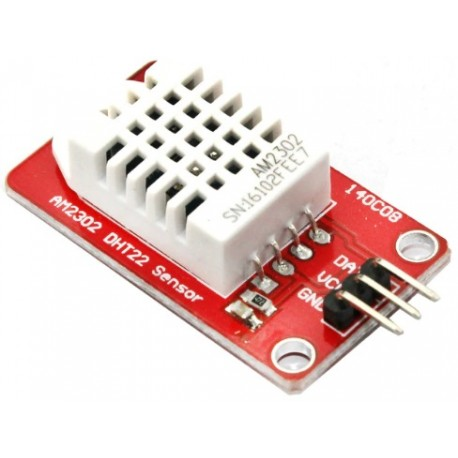
\includegraphics[width=5cm, height=5cm]{imagenes/dht22.jpg}
      \caption{Sensor DHT22}
      \subcaption*{Fuente: Datasheet fabricante}
      \label{imag:dht22}
   \end{figure}
   
El DHT22 (AM2302) es un sensor digital de temperatura y humedad relativa de buen rendimiento y de bajo costo. Integra un sensor capacitivo de humedad y un termistor para medir el aire circundante, y muestra los datos mediante una señal digital en el pin de datos (no posee salida analógica).\\

\begin{figure}[H]
    \centering
    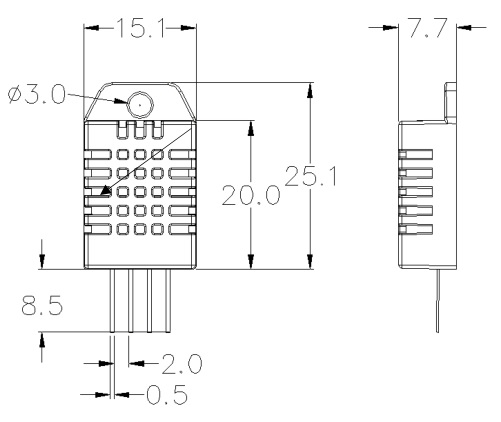
\includegraphics[width=8cm, height=6cm]{imagenes/dht22 dimensiones.jpg}
    \caption{Dimensiones sensor DHT22}
    \subcaption*{Fuente: Datasheet fabricante}
    \label{imag:dimensiones_dht22}
\end{figure}

\vspace{1cm}

\addcontentsline{toc}{subsection}{\hspace{1.3cm}2.2.1.2\hspace{5mm}Sensor MZ-Z19C}
        \textbf{2.2.1.2\hspace{5mm}Sensor MZ-Z19C}

\begin{figure}[H]
      \centering
      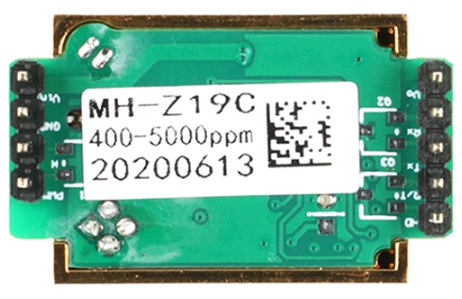
\includegraphics[width=5cm, height=3cm]{imagenes/mh-z19c.png}
      \caption{Sensor MH-Z19C}
      \label{imag:mh-z19c}
   \end{figure}

El sensor de gas de dióxido de carbono MH-Z19C es un pequeño sensor inteligente de uso general que utiliza el principio del infrarrojo no disperso (NDIR) para detectar la presencia de CO2 en el aire.\\\\

\textbf{Otros datos}
\begin{itemize}
    \item Señal de salida: UART(TTL)
    \item Tiempo de precalentamiento: 60 segundos
    \item Temperatura de operación: De -10 a 50°C
    \item Humedad de operación: De 0 - 95 por ciento RH
    \item Dimensiones: aprox. 39 x 20 x 9 mm
    \item Tipo de conector: JST ZH de 7 pines
\end{itemize}

\vspace{0.5cm}

\addcontentsline{toc}{subsection}{\hspace{1.3cm}2.2.1.3\hspace{5mm}Sensor M0168}
        \textbf{2.2.1.3\hspace{5mm}Sensor M0168}

\begin{figure}[H]
      \centering
      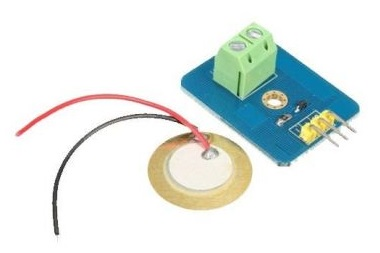
\includegraphics[width=6.5cm, height=5cm]{imagenes/sensor-piezoelectrico.jpg}
      \caption{Sensor piezoeléctrico M0168}
      \label{imag:M0168}
   \end{figure}

En este sensor piezoeléctrico cuando el choque de la cerámica con la lámina metálica genera una señal eléctrica, esta señal analógica es la recibida por los pines analógicos de microcontroladores.\\

\textbf{Especificaciones Técnicas}

\begin{itemize}
    \item Voltaje de trabajo: 3.3V o 5V
    \item Corriente de trabajo: 1mA
    \item Rango de temperatura de funcionamiento: -10 ~ +70
    \item Interfaz Tipo: salida analógica
    \item Tamaño del artículo: 30mm x 23mm
\end{itemize}

\addcontentsline{toc}{subsection}{\hspace{1.3cm}2.2.1.4\hspace{5mm}Sensor SDS011}
        \textbf{2.2.1.4\hspace{5mm}Sensor SDS011}

\vspace{1cm}

\begin{figure}[H]
      \centering
      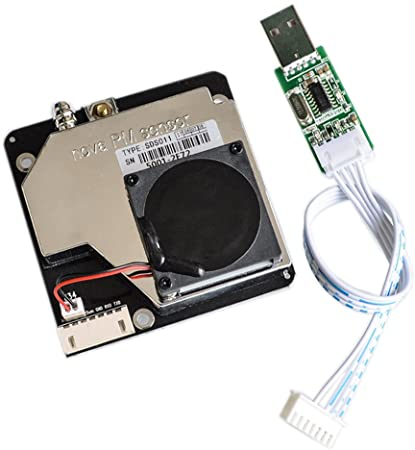
\includegraphics[width=4.5cm, height=4.5cm]{imagenes/Sensor SDS011.jpg}
      \caption{Sensor SDS011}
      \label{imag:SDS011}
   \end{figure}

Se basa en el principio de dispersión láser: se puede inducir la dispersión de la luz cuando las partículas atraviesan el área de detección. La luz dispersa se transforma en señales eléctricas, después estas señales serán amplificadas y procesadas. El número y el diámetro de las partículas se pueden obtener mediante análisis porque la forma de onda tiene ciertas relaciones con el diámetro de las partículas.\\

\textbf{Otros datos}

\begin{itemize}
    \item Corriente del sueño: 2mA
    \item Frecuencia de muestreo serie: 1 segundo
    \item Resolución diámetro de partículas: <= 0.3um
    \item Rango de temperatura: -20 a 50°C
    \item Tamaño físico: 71mm x 70mm x 23mm 
\end{itemize}

\vspace{5cm}

\addcontentsline{toc}{subsection}{\hspace{1.3cm}2.2.1.5\hspace{5mm}Sensor LDR}
        \textbf{2.2.1.5\hspace{5mm}Sensor LDR}\newline

\begin{figure}[H]
      \centering
      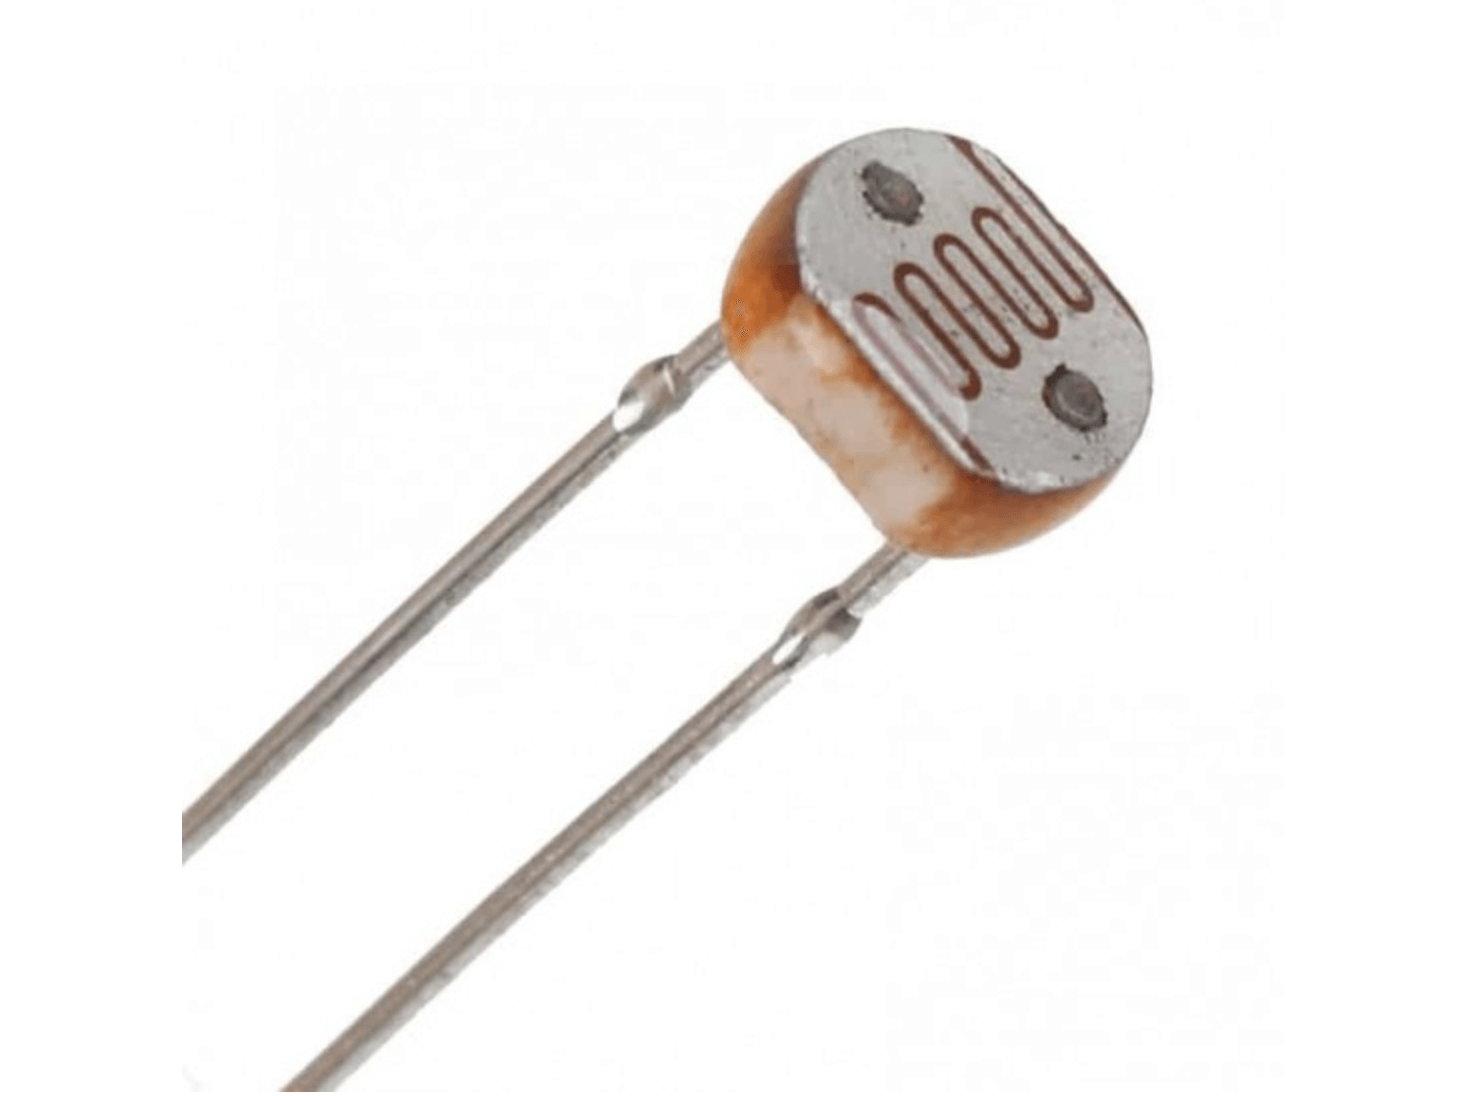
\includegraphics[width=5.5cm, height=4cm]{imagenes/sensor LDR.png}
      \caption{Sensor LDR}
      \label{imag:LDR}
   \end{figure}

Una fotorresistencia es un componente electrónico cuya resistencia disminuye con el aumento de la intensidad de la luz incidente. Puede también ser llamado fotorresistor, fotoconductor, célula fotoeléctrica o resistor dependiente de la luz, cuyas siglas, LDR, se originan de su nombre en inglés light-dependent resistor.\\

\begin{figure}[H]
    \centering
    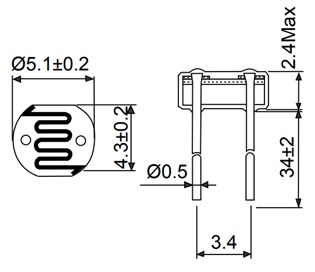
\includegraphics[width=4.5cm, height=4cm]{imagenes/ldr.jpg}
    \caption{Sensor LDR}
    \subcaption*{Fuente: Datasheet fabricante}
    \label{imag:dimensiones LDR}
 \end{figure}

\vspace{0.5cm}

\addcontentsline{toc}{subsection}{\hspace{1.3cm}2.2.1.6\hspace{5mm}Sensor BH1750}
        \textbf{2.2.1.6\hspace{5mm}Sensor BH1750}\newline

El Módulo BH1750 es un sensor de iluminación digital para medición de flujo luminoso (iluminancia) de la empresa Rohm Semiconductor. Componente que posee dentro de su arquitectura interna, un conversor análogo digital (ADC) de 16 bits con una salida digital de formato I2C, que facilita la integración con microcontroladores o sistemas embebidos diversos. Este módulo entrega la intensidad luminosa directamente en unidades de Lux que es equivalente a Lumen/m2.\\

\begin{figure}[H]
    \centering
    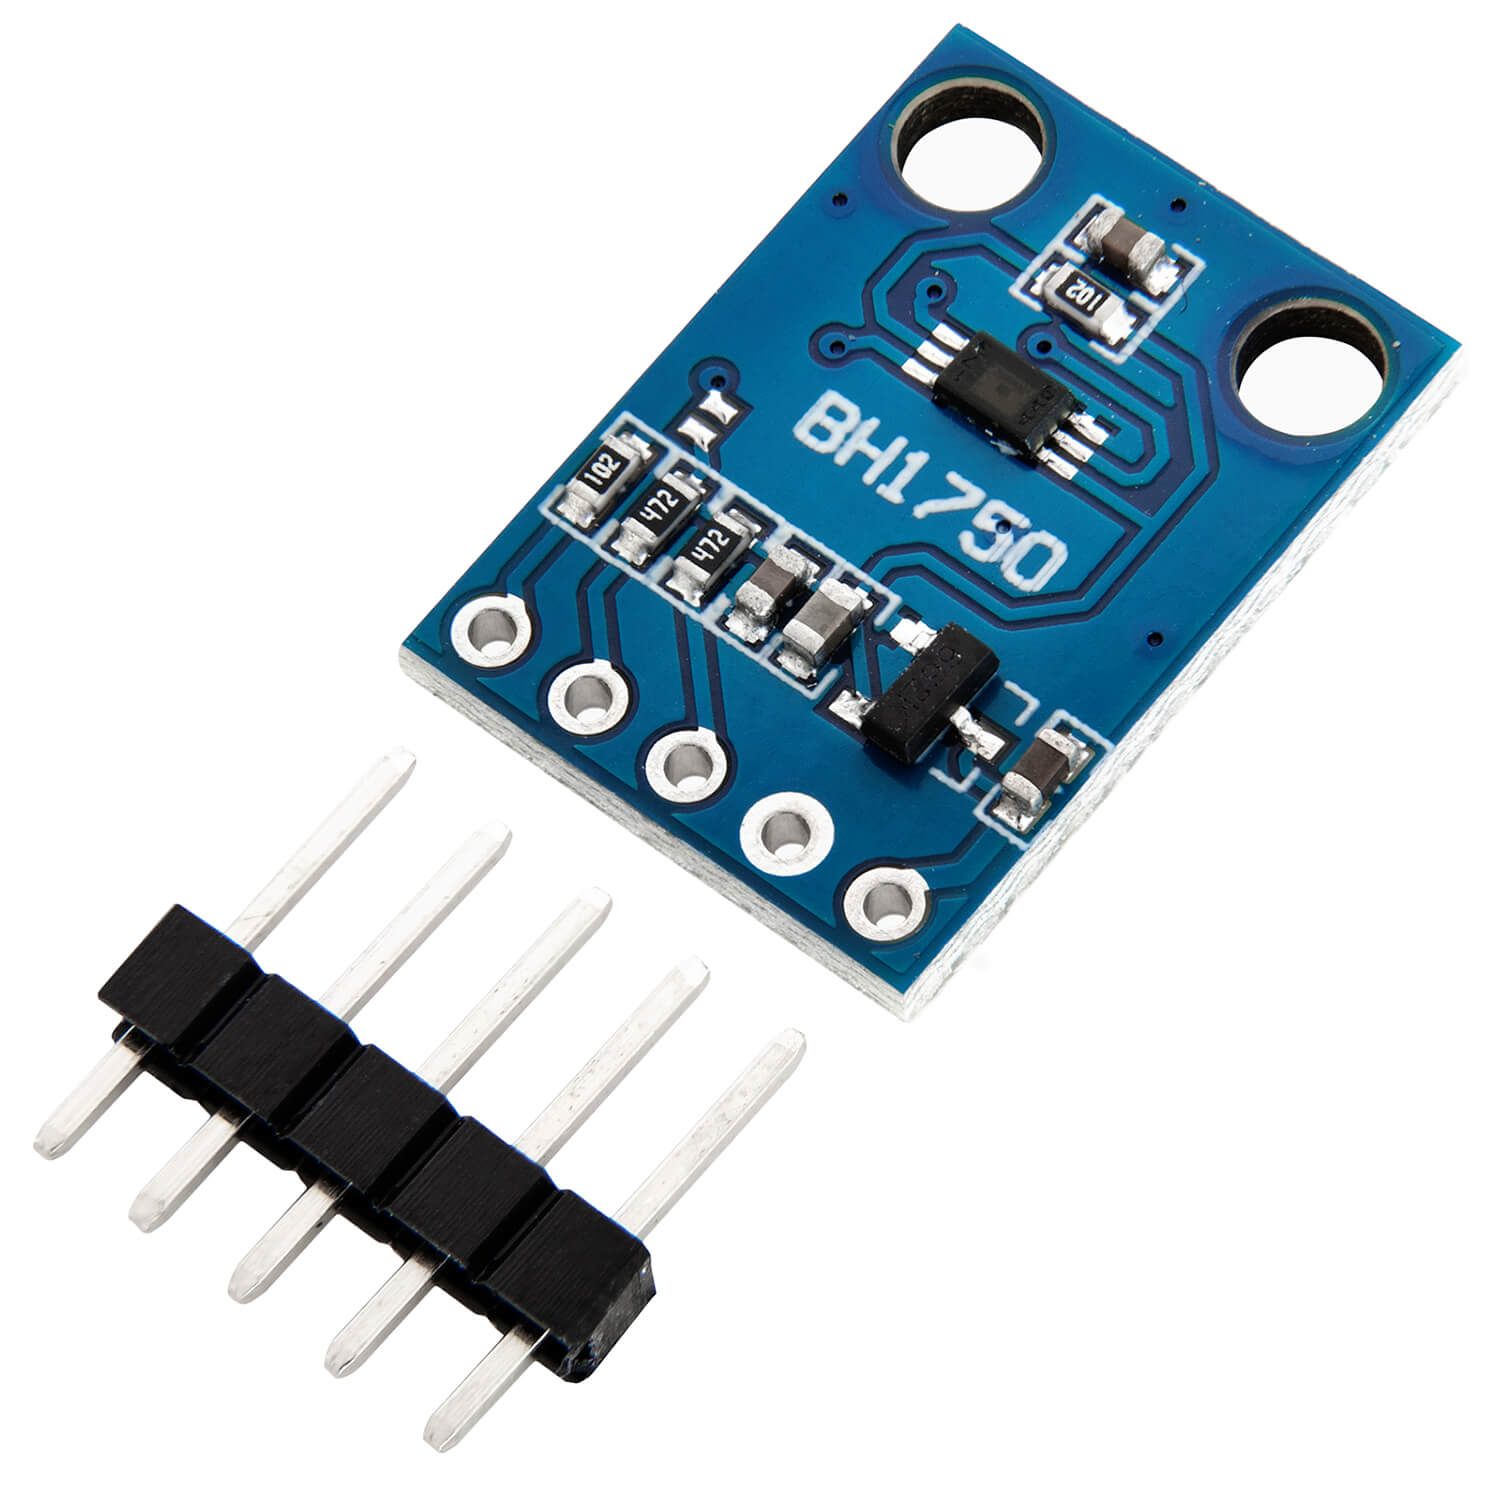
\includegraphics[width=5cm, height=4cm]{imagenes/Sensor BH1750.jpg}
    \caption{Sensor BH1750}
    \label{imag:BH1750}
 \end{figure}

\textbf{Otros datos}

\begin{itemize}
    \item Interfaz Digital: I2C
    \item Frecuencia máxima de transmisión: 400kHZ
    \item Temperatura de operación: Desde -40°C hasta 85°C
\end{itemize}

Para su correcto funcionamiento, este sensor debe ir acompañado de una serie de componentes electrónicos para su acondicionamiento.
En la figura \ref{imag:acondicionamiento_BH1750} se puede observar el acondicionamiento brindado por el fabricante.

\begin{figure}[H]
    \centering
    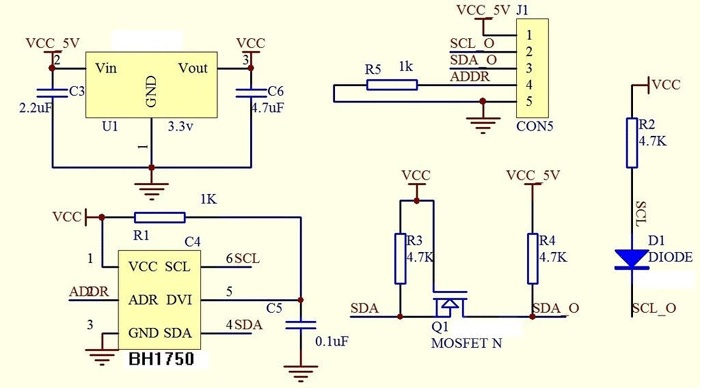
\includegraphics[width=11cm, height=7cm]{imagenes/acondicionamientos sensor BH1750.jpg}
    \caption{Acondicionamiento sensor BH1750}
    \subcaption*{Fuente: Datasheet fabricante}
    \label{imag:acondicionamiento_BH1750}
\end{figure}

\vspace{1cm}

\subsection{Alimentación}

\textbf{Regulador LDO RT9013.}\newline

Información obtenida del Datasheet que ofrece el fabricante...\\

The RT9013 is a high-performance, 500mA LDO regulator, offering extremely high PSRR and ultra-low dropout. Ideal for portable RF and wireless applications with demanding performance and space requirements.\\

The RT9013 quiescent current as low as 25uA, further prolonging the battery life. The RT9013 also works with low-ESR ceramic capacitors, reducing the amount of board space necessary for power applications, critical in handheld wireless devices.\\

The RT9013 consumes typical 0.7uA in shutdown mode and has fast turn-on time less than 40us. The other features include ultra-low dropout voltage, high output accuracy, current limiting protection, and high ripple rejection ratio. Available in the SC-82, SOT-23-5, SC-70-5 and WDFN-6L 2x2 package.\\

\textbf{Características}

\begin{itemize}
    \item Wide Operating Voltage Ranges : 2.2V to 5.5V
    \item Low Dropout : 250mV at 500mA
    \item Ultra-Low-Noise for RF Application
    \item Ultra-Fast Response in Line/Load Transient
    \item Current Limiting Protection
    \item Thermal Shutdown Protection
    \item High Power Supply Rejection Ratio
    \item Output Only 1 uF Capacitor Required for Stability
    \item TTL-Logic-Controlled Shutdown Input
\end{itemize}

\vspace{1cm}

\begin{figure}[H]
    \centering
    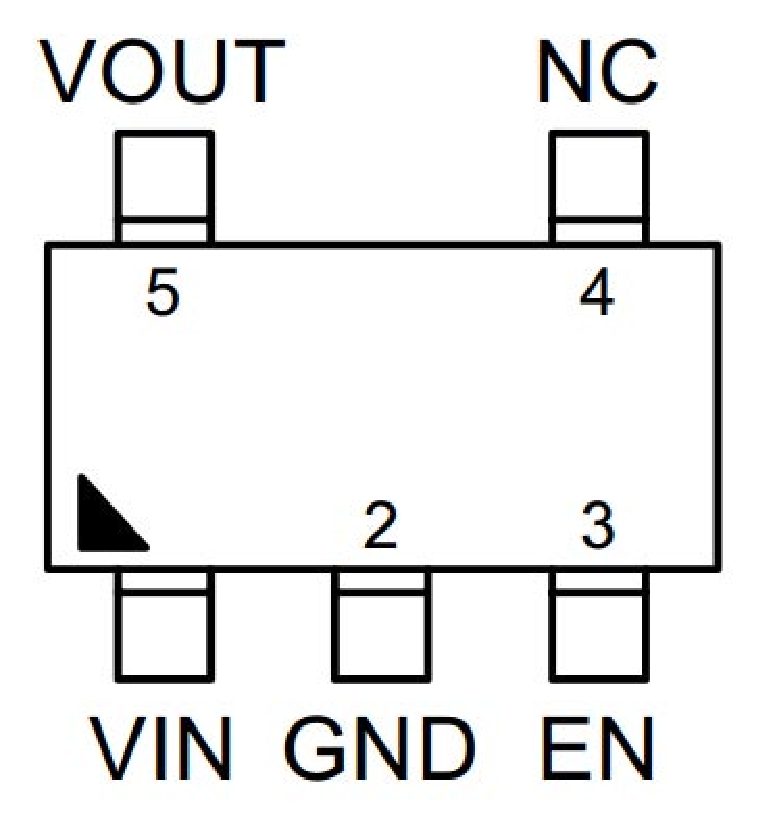
\includegraphics[width=5.5cm, height=6cm]{imagenes/esquematico RT9013.pdf}
    \caption{Configuración de pines}
    \subcaption*{Fuente: Datasheet fabricante}
    \label{imag:pines_RT9013}
\end{figure}

\begin{figure}[H]
    \centering
    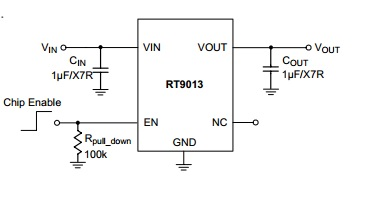
\includegraphics[width=12cm, height=7cm]{imagenes/acondicionamiento RT9013.jpg}
    \caption{Acondicionamiento}
    \subcaption*{Fuente: Datasheet fabricante}
    \label{imag:acondicionamiento_RT9013}
\end{figure}


\addcontentsline{toc}{section}{Conclusiones}
        \textbf{\Large Conclusiones}\newline
